\documentclass{fefu}

\usepackage{graphicx}
\usepackage{float}
\usepackage{wrapfig}

\begin{document}
	\setschool{ШКОЛА ЕСТЕСТВЕННЫХ НАУК}
	\setdepartment{кафедра информатики, математического и компьютерного 
	моделирования}{А.Ю.Чеботарев}
	\setgroup{Б8403а}
	\title{о прохождении преддипломной практики\\направление подготовки 01.03.02 
	Прикладная математика и информатика\\профиль «Системное программирование»}
	\setdates{29}{апреля}{2019}{22}{июня}{2019}
	\setweeks{8}
	\setplace{кафедре информатики, \\математического и компьютерного \\моделирования}
	\author{Куцелабский Е.С.}
	\setsupervisor{Кленин А.С.}
	
	\makereporttitle
	\tableofcontents
	\newpage

	\section*{Введение}
		\par Преддипломная практика - заключительный этап подготовки к написанию выпускной
		квалификационной работы и к работе по специальности. Благодаря ей студент
		может ознакомиться с будущей профессией не только теоретически, но и на практике.
		\par Актуальность практики продиктована необходимостью обобщения, актуализации и
		систематизации полученных за время обучения теоретических знаний.
		\par Целью преддипломной практики является разработка текстового процессора для 
		open-source движка Citrus.
		\par Сроки прохождения практики: с 29 апреля 2019 по 22 июня 2019 (общая длительность 
		-- 8 недель).
		\par За время практики требуется выполнить следующие задачи: 
		\begin{enumerate}
			\item Изучить имеющиеся подходы к реализации текстовых редакторов
			\item Создать редактор, обеспечивающий:
			\begin{itemize}
				\setlength{\itemindent}{-3em}
				\item Просмотр и редактирование обычного (не стилизованного) текста
				\item Поддержку работы с многострочными файлами
				\item Эффективную отрисовку больших объемов текста
				\item Поддержку стандартных пользовательских команд
			\end{itemize}
			\item Сравнить производительность новой и старой версий редактора
		\end{enumerate}
        \par Для их достижения был составлен план работ:
		\begin{enumerate}
			\item Изучение подходов к реализации текстовых редакторов (1-2 недели)
			\item Изучение кодовой базы движка Citrus в целях нахождения места для внесения
			изменений (1 неделя)
			\item Реализация текстового редактора (4 недели)
			\item Подготовка отчёта (1 неделя)
		\end{enumerate}
		\section{Описание предметной области}
			\subsection{Студия Game Forest}
				\par Данная работа выполняется для студии Game Forest. \cite{GFPortal} 
				Студия занимается созданием игр, и за время своего существования выпустила 
				более 40 проектов, суммарная аудитория которых -- более 100 млн человек. 
				Игровые проекты получали высокие оценки игроков, критиков и издателей, наиболее 
				успешной игрой, в данный момент, является Gummy Drop (количество скачиваний -- 
				более 50 млн)\cite{GummyDropPage}.
				\par Основой игровых проектов, в данный момент, является разработка студии -- 
				игровой движок Citrus. Он позволяет создавать приложения для нескольких
				платформ: Windows, MacOS, Android, iOS.
				\par Несмотря на существование крупных открытых игровых движков, таких как 
				Unity \cite{UnitySite} и Unreal Engine \cite{UnrealEngineSite}, 
				в Game Forest было принято решение использовать собственную разработку. К 
				такому же решению пришли многие крупные компании, например, Bethesda Game 
				Studios \cite{BethesdaEngine} и id Software \cite{idSoftwareEngine}.
				\par Крупные движки содержат инструменты для разработки игр всех жанров. 
				Создание и поддержка подобных инструментов даже на базовом уровне требует 
				огромных усилий, а учитывая тот факт, что подобные движки рассчитаны
				на массовую (часто непрофессиональную) аудиторию, комфорт и простота
				использования ставятся превыше производительности, что отрицательно сказывается
				на конечном продукте. Именно поэтому компании принимают решение о разработке
				собственных движков, создаваемых с учетом нужд компании. В подобных движках
				отсутствуют лишние компоненты, присущие массовым движкам, что позволяет
				сосредоточиться на улучшении действительно важных частей системы.
				\par Стоит отметить, что, в отличие от конкурентов, студия Game
				Forest распространяет свой движок под лицензией GPL-3.0, что позволяет
				использование, модификацию и распространение движка другими студиями и
				отдельными пользователями.
			\subsection{Игровой движок Citrus}
				\par Citrus состоит из нескольких взаимосвязанных модулей, каждый из которых
				реализует определенную функциональность (см. Рис. \ref{img:CitrusScheme})
				\cite{CitrusRepo}: 
				\begin{itemize}
					\item Yuzu --- библиотека, предоставляющая средства сериализации
					\item Kumquat --- генератор кода
					\item Lemon --- модуль компоновки сторонних библиотек
					\item Lime --- ядро движка
					\item Orange --- сборщик проектов, созданных при помощи движка
					\item Tangerine --- редактор сцен
				\end{itemize}
				\par Движок предоставляет возможность визуализации 2D и 3D графики, 
				оконных интерфейсов, поддерживает воспроизведение звуков, сборку проектов для 
				нескольких платформ, проигрывание и редактирование анимаций (в визуальном 
				редакторе). Компоненты активно дорабатываются, набор поддерживаемых функций, 
				при необходимости, дополняется.
				\par В модуле Lime, помимо прочего, содержатся части системы, ответственные за
				работу с текстом.
				\begin{figure}[h]
					\centering
					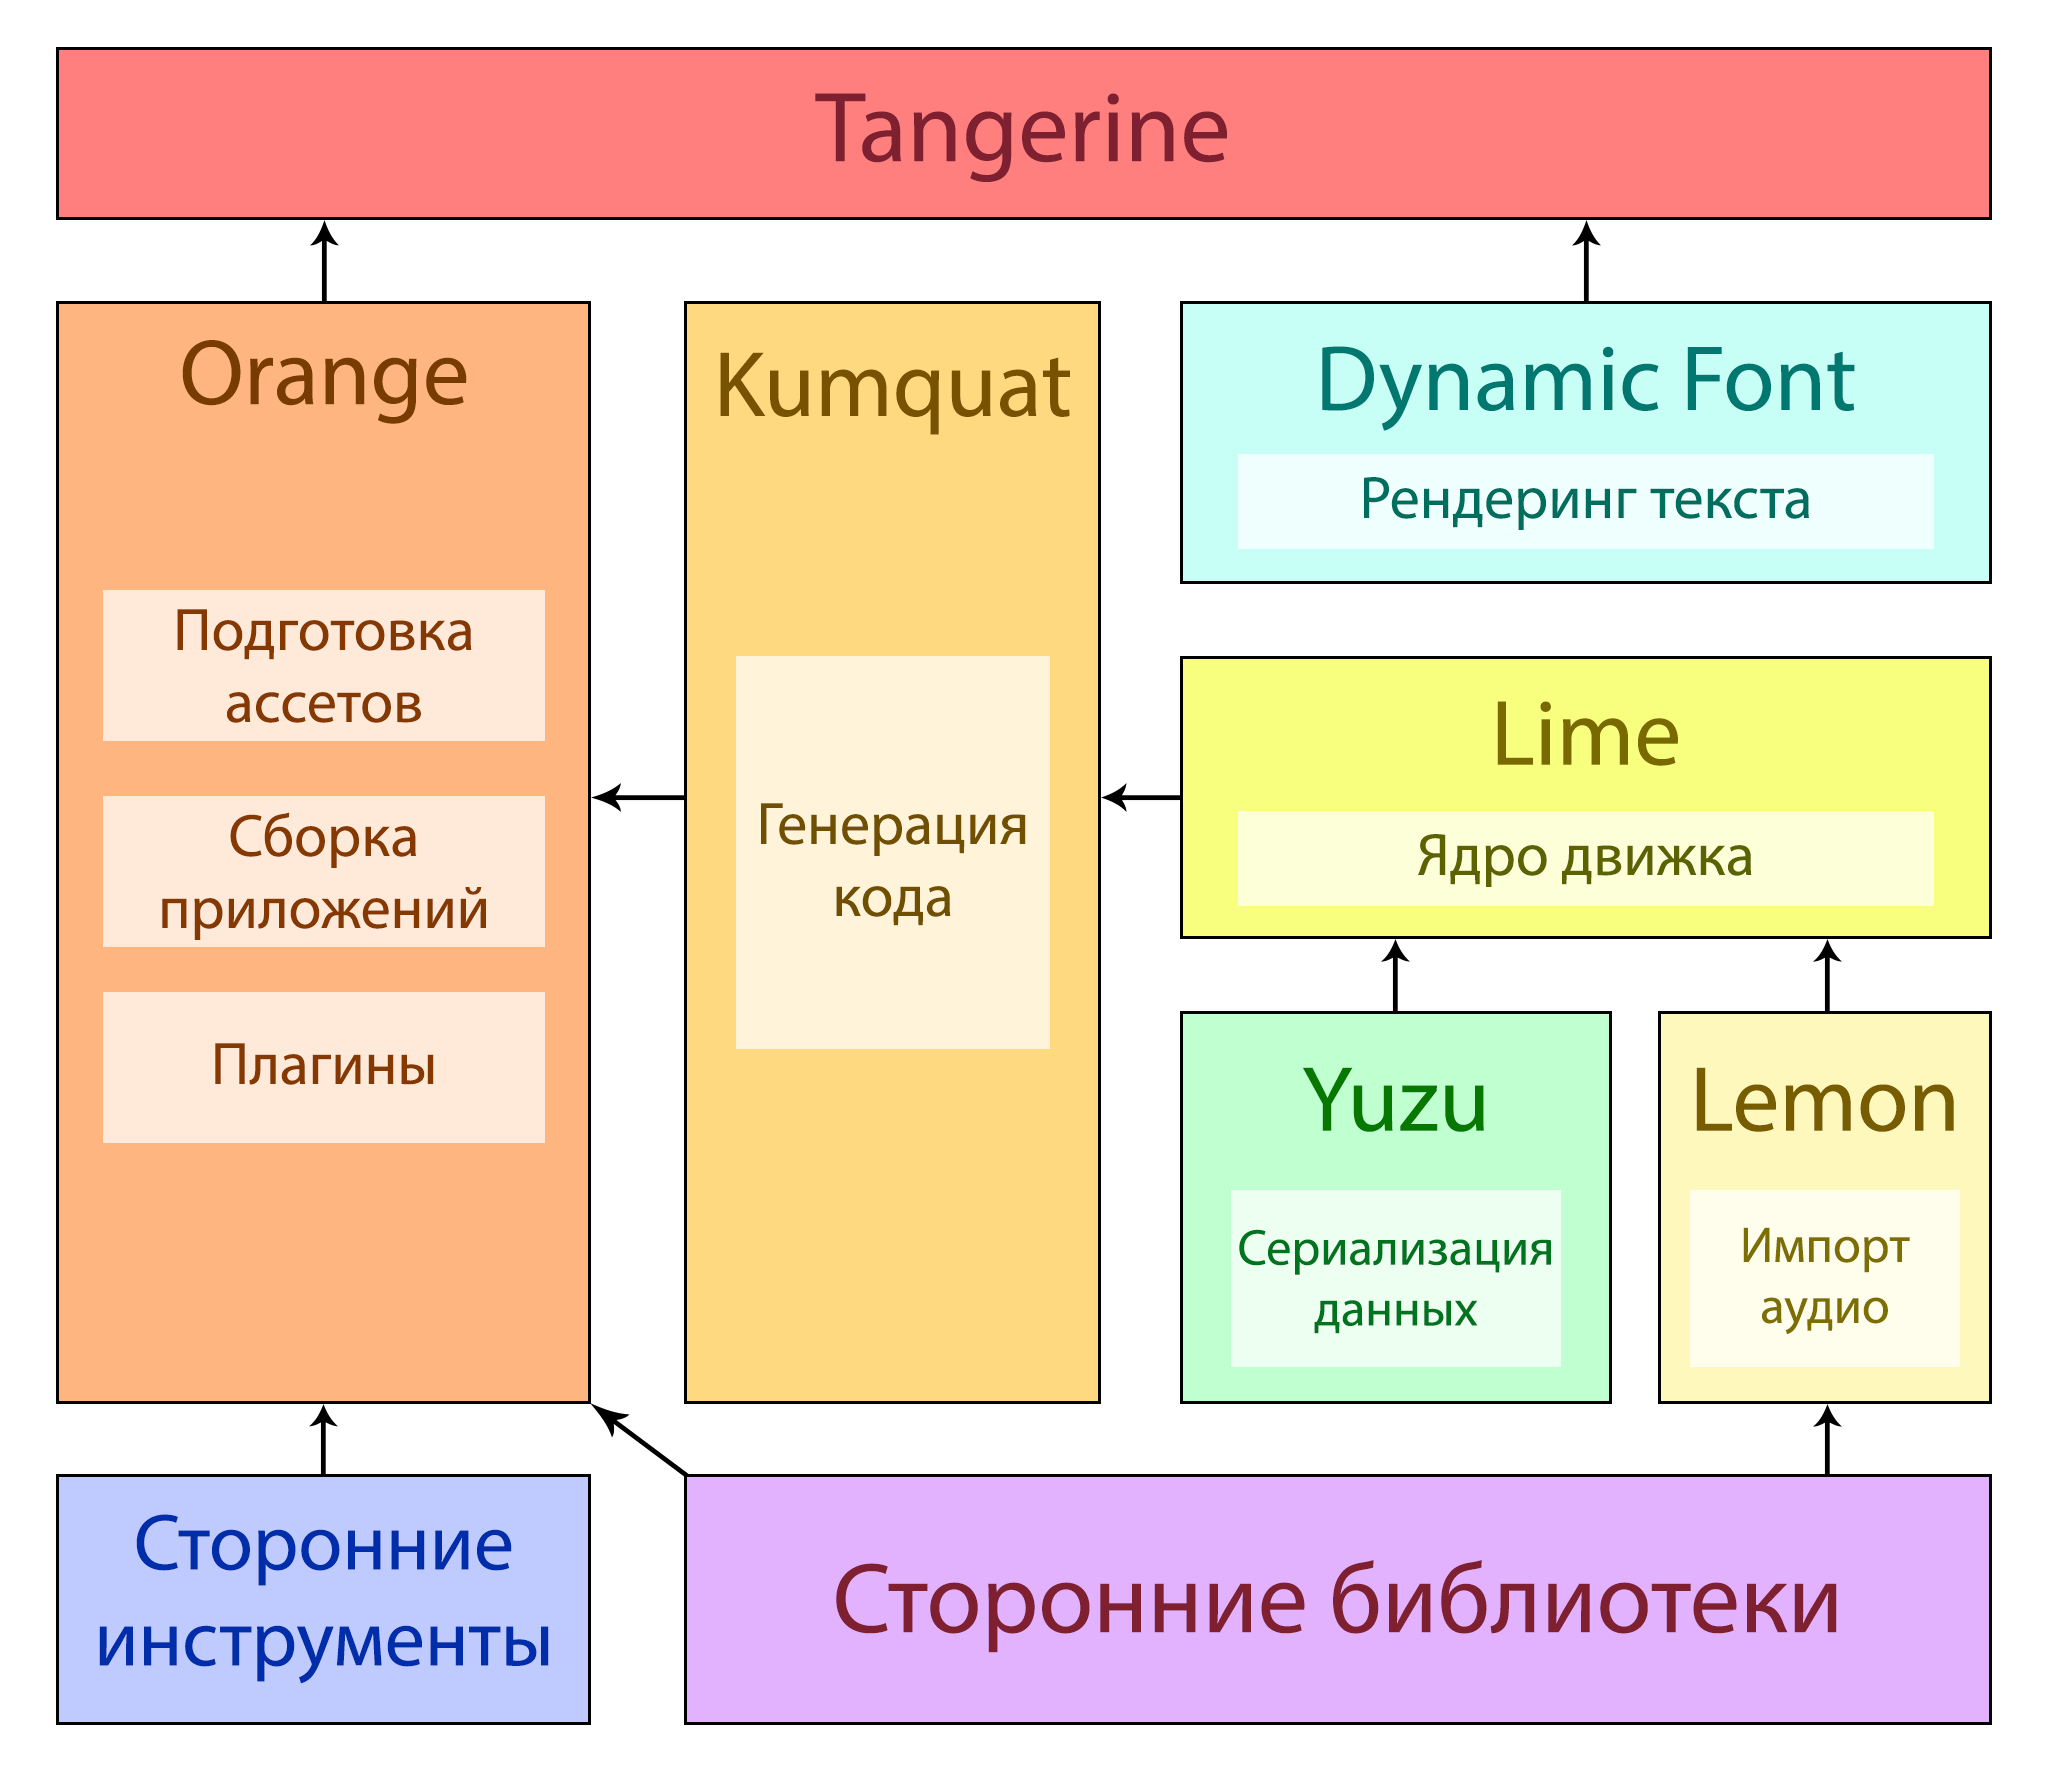
\includegraphics[width=1\linewidth]{images/CitrusScheme.png}
					\caption{Схема модулей движка Citrus}
					\label{img:CitrusScheme}
				\end{figure}
				%\par \textbf{Добавить огромное количество инфы про цитрус}
			\subsection{Текстовый редактор}
				\par Текстовый редактор это компьютерная программа (или её часть), 
				предназначенная для создания и изменения текстовых данных (в том числе 
				текстовых файлов). Часто редакторы предоставляют пользователям дополнительные 
				возможности, такие как: копирование и вставка, поиск и замена текста, 
				форматирование текста (переносы строк, выравнивание и пр.), 
				откат/восстановление изменений \cite{WhatIsATextEditor}. 
				\par Некоторые редакторы, помимо работы с обычным текстом, позволяют также и
				работу со стилизованным текстом (т.н. Rich Text) 
				\cite{DiffBetweenTextFormats}. Так как текстовый формат данных не предполагает
				хранения информации о стиле текста, в редакторах тексты обрамляются в различные
				языки разметки (например, HTML), либо используется внутреннее двоичное 
				представление.
				\par Для успешной работы текстового редактора необходимо, чтобы были
				реализованы три его основные компоненты: \cite{CraftOfTextEditing}
				\begin{enumerate}
					\item Обработка внутреннего представления текста --- текст необходимо
					эффективным образом хранить и изменять, наивный подход к этой части
					редактора приведёт к значительному (в случае работы с большими объемами
					данных -- к фатальному) падению производительности всего редактора.
					\item Отрисовка --- текст необходимо правильно отрисовать с учетом размеров
					окна и применённых стилей (шрифт, выравнивание, переносы слов).
					\item Обработка пользовательского ввода --- приём команд
					(вставка, удаление элемента, перевод курсора и~пр.) и передача их
					обработчику внутреннего представления.
				\end{enumerate}
			\subsection{Обработка текста в Citrus}
				\par Представление текстовых данных и работа с ними -- важная часть игрового
				движка, поскольку значительная часть важной игровой информации сообщается 
				пользователю в текстовом виде. 
				%\textbf{Вставить инфу о классах, занимающихся
				%текстом (IText, RichText, SimpleText, TextParser, TextStyle, TextRenderer,
				%Editor)} 
				В Citrus есть классы, обеспечивающие обработку ввода и отрисовку текста, 
				однако они реализованы неэффективно, что выражается в резком падении 
				производительности с увеличением длины текста. Это приводит к увеличению
				требований к процессору для поддержания высокой частоты кадров. При дальнейшем
				увеличении объема текста работа программ сильно замедляется, что критично для
				игровых проектов, и составляет значительные неудобства при работе со средствами
				визуального редактирования в движке. Также стоит отметить, что несмотря на
				возможность корректно отображать многострочный текст, текущая система слабо
				приспособлена для его редактирования.
				\par В данный момент эти проблемы решаются обходным путём, т.е. число
				использований многострочного редактора сведено к минимуму, а появления больших
				объемов текста стараются, по возможности, не допускать. В игровых проектах
				число больших текстов невелико, а во время работы с визуальной частью движка
				неэффективность работы текстовой системы, хоть и замедляет работу, не является
				критическим препятствием.
				\par Для решения данных проблем можно переписать всю систему работы с текстом с
				нуля, а можно лишь оптимизировать малоэффективные части. Поскольку разработка 
				подобной системы связана со значительными трудностями, в то время как на уже
				существующую систему опираются многие игровые проекты, я решил лишь внести 
				необходимые изменения в существующую структуру работы.
				\par Первую часть системы -- обработку внутреннего представления текста -- 
				можно использовать как самостоятельную единицу в любых других проектах. Все 
				прочие части завязаны на существующую архитектуру движка Citrus и без него 
				неприменимы.
	\section{Подход к реализации}
				\par Таблица кусочков (Piece Table) - эффективная структура данных, используемая во многих современных 
				текстовых редакторах \cite{PieceTableArticle}. Используется несколько потоков
				(файлов) -- исходный и добавочный. Исходный поток используется только для 
				чтения. В добавочный данные добавляются и читаются из него, но не удаляются.
				Вместо хранения самих символов, в структуре хранится информация о текстовых 
				фрагментах, а именно: позиция начала фрагмента в потоке (файле), его длина, 
				исходный ли это поток или добавочный. При добавлении новых символов они
				записываются в добавочный поток, а в таблицу заносится новый фрагмент. При
				вставке текста, в случае если позиция нового фрагмента содержится внутри
				существующего, возможно разбиение фрагментов на две части, тогда в левой части
				фрагмента остаётся информация о части текста, лежащей до нового фрагмента, а в 
				правой -- после. Во время удаления от фрагментов "отрезаются" части, либо весь
				фрагмент удаляется целиком.
				\par Таблица кусочков это лишь структура данных для хранения информации о
				тексте, настоящую эффективность данному подходу придаёт способ хранения
				кусочков. Одним из наиболее эффективных способов является использование 
				расширяющегося дерева (Splay Tree). Это сбалансированное бинарное дерево 
				поиска, в котором элементы, к которым в последний раз было произведено
				обращение, перемещаются в корень. Это свойство особенно эффективно при
				использовании в текстовых редакторах, поскольку в них большая часть изменений
				производится около одного места -- позиции курсора \cite{SplayTreeArticle}.
				\par При использовании расширяющегося дерева сложность вставки и удаления
				составляет $O(log~m)$, где $m$ -- число фрагментов в дереве. Операция получения
				элемента так же выполняется за $O(log~m)$, однако стоит учесть, что
				требуются дополнительные затраты времени на чтение данных из потока.
				\par Операция получения элемента по номерам строки и столбца в случае наивной
				реализации имеет сложность $O(n)$, где $n$ -- число символов в тексте, однако
				зачастую применяются различные техники для оптимизации этой операции.
				\par Все вышеперечисленные сложности описаны для худшего случая, в случае
				работы с текстом в позиции курсора операции будут выполнены значительно 
				быстрее, поскольку все необходимые элементы будут находиться близко к корню
				дерева, благодаря чему для достижения нужной позиции не потребуется совершать
				полный пробег по дереву.
				\par Дополнительным преимуществом подхода является тот факт, что он
				использует значительно меньше памяти, чем прочие, поскольку вместо хранения,
				непосредственно, символов, хранится лишь набор ссылок на части текста.
				%\textbf{Вставить картинку}
	\section{Архитектура системы}
		\par Систему можно поделить на три модуля:
		\begin{enumerate}
			\item Модуль обработки внутреннего представления текста --- отвечает за хранение
			текста и эффективное выполнение базовых операций (вставка, удаление, доступ).
			\item Модуль отрисовки --- обеспечивает корректную и эффективную отрисовку текста
			с учетом размеров виджета.
			\item Модуль обработки пользовательского ввода --- отвечает за получение
			пользовательских команд и отправку их в обработчик внутреннего представления.
		\end{enumerate}
			\subsection{Обработка внутреннего представления текста}
				\par Данный модуль состоит из следующих классов:
				\begin{itemize}
					\item CaretPosition --- описывает положение курсора и 
					обрабатывает его перемещение.
					\item Selection --- хранит информацию о текущем выделении, обрабатывает его
					изменения
					\item UndoStack --- хранит стек обработанных операций, по запросу PieceTree 
					сообщает необходимые данные 
					\item SubEditor --- связующее звено между модулями. Принимает команды на 
					редактирование текста и перемещение курсора, перенаправляет их
					соответствующим модулям
				\end{itemize}
			\subsection{Модуль отрисовки}
				\par Данный модуль состоит из следующих классов:
				\begin{itemize}
					\item TextParser --- выделяет из текста фрагменты (отдельные слова, 
					переносы строк, пробелы)
					\item TextRenderer --- получает набор фрагментов от TextParser, для каждого
					фрагмента определяет его позицию в тексте, учитывая параметры шрифта и 
					размеры окна, при необходимости применяет soft wrap, затем передаёт
					полученные данные в общий рендерер движка, который выполняет
					непосредственную отрисовку
					\item CommonText --- содержит в себе SubEditor, TextParser и TextRenderer,
					обеспечивает обмен данными между ними, помимо этого содержит информацию о
					параметрах шрифта. Стоит отметить, что в случаях, когда необходимо лишь 
					отобразить текст без возможности редактирования, достаточно возможностей
					этого класса
				\end{itemize}
			\subsection{Модуль обработки пользовательского ввода}
				\par Вся функциональность данного модуля содержится в классе Editor. Он
				обрабатывает пользовательский ввод, перенаправляя команды в SubEditor,
				находящийся внутри CommonText, который является полем в Editor.
				%\textbf{В доме, который построил Джек. Надо бы перефразировать.}
		\section{Вычислительный эксперимент}
			\par Было проведено ручное сравнение производительности предыдущей и новой версий 
			редактора. Тестирование проводилось на тексте объемом 100 тысяч строк.
			\par Тестирование показало, что при вертикальной прокрутке новый вариант редактора
			редактора отрисовывает текст без задержки на высокой частоте кадров, в то время как
			старая версия показывает новый кадр с задержкой в 2-3 секунды.
	\section*{Заключение}
		\par В ходе практики все поставленные задачи были выполнены согласно плану работ.
		Были исследованы методы реализации текстовых процессоров, выбран и реализован
		эффективный подход, проведён вычислительный эксперимент, углублены знания в языке 
		программирования C\# и в методах автоматического тестирования.
		\par Со стороны руководителя практики была оказана значительная помощь в изучении
		предметной области и выполнении практических задач.
	\newpage
	\bibliographystyle{ugost2008ls}
	\bibliography{references}	
\end{document}